%%%%%%%%%%%%%%%%%%%%%%%%%%%%%%%%%%%%%%%%%%%%%%%%%%%%%%%%%%%%%%%%%%%%%%%%%%%%
% AGUJournalTemplate.tex: this template file is for articles formatted with LaTeX
%
% This file includes commands and instructions
% given in the order necessary to produce a final output that will
% satisfy AGU requirements, including customized APA reference formatting.
%
% You may copy this file and give it your
% article name, and enter your text.
%
%
% Step 1: Set the \documentclass
%
%

%% To submit your paper:
\documentclass[draft]{agujournal2019}
\usepackage{url} %this package should fix any errors with URLs in refs.
\usepackage{lineno}
\usepackage[inline]{trackchanges} %for better track changes. finalnew option will compile document with changes incorporated.
\usepackage{soul}
\usepackage{subfigure}
\linenumbers
%%%%%%%
% As of 2018 we recommend use of the TrackChanges package to mark revisions.
% The trackchanges package adds five new LaTeX commands:
%
%  \note[editor]{The note}
%  \annote[editor]{Text to annotate}{The note}
%  \add[editor]{Text to add}
%  \remove[editor]{Text to remove}
%  \change[editor]{Text to remove}{Text to add}
%
% complete documentation is here: http://trackchanges.sourceforge.net/
%%%%%%%

\draftfalse

%% Enter journal name below.
%% Choose from this list of Journals:
%
% JGR: Atmospheres
% JGR: Biogeosciences
% JGR: Earth Surface
% JGR: Oceans
% JGR: Planets
% JGR: Solid Earth
% JGR: Space Physics
% Global Biogeochemical Cycles
% Geophysical Research Letters
% Paleoceanography and Paleoclimatology
% Radio Science
% Reviews of Geophysics
% Tectonics
% Space Weather
% Water Resources Research
% Geochemistry, Geophysics, Geosystems
% Journal of Advances in Modeling Earth Systems (JAMES)
% Earth's Future
% Earth and Space Science
% Geohealth
%
% ie, \journalname{Water Resources Research}

\journalname{Enter journal name here}


\begin{document}

%% ------------------------------------------------------------------------ %%
%  Title
%
% (A title should be specific, informative, and brief. Use
% abbreviations only if they are defined in the abstract. Titles that
% start with general keywords then specific terms are optimized in
% searches)
%
%% ------------------------------------------------------------------------ %%

% Example: \title{This is a test title}

\title{Application of Empirical Mode Decomposition of cosmic ray in prediction of great geomagnetic storms}

%% ------------------------------------------------------------------------ %%
%
%  AUTHORS AND AFFILIATIONS
%
%% ------------------------------------------------------------------------ %%

% Authors are individuals who have significantly contributed to the
% research and preparation of the article. Group authors are allowed, if
% each author in the group is separately identified in an appendix.)

% List authors by first name or initial followed by last name and
% separated by commas. Use \affil{} to number affiliations, and
% \thanks{} for author notes.
% Additional author notes should be indicated with \thanks{} (for
% example, for current addresses).

% Example: \authors{A. B. Author\affil{1}\thanks{Current address, Antartica}, B. C. Author\affil{2,3}, and D. E.
% Author\affil{3,4}\thanks{Also funded by Monsanto.}}

\authors{Cong Wang\affil{1},Qian Ye\affil{1},BingSen Xue\affil{1}}


% \affiliation{1}{First Affiliation}
% \affiliation{2}{Second Affiliation}
% \affiliation{3}{Third Affiliation}
% \affiliation{4}{Fourth Affiliation}

\affiliation{1}{Key Laboratory for Space Weather, National Center for Space Weather, Beijing 100029, China}
%(repeat as many times as is necessary)

%% Corresponding Author:
% Corresponding author mailing address and e-mail address:

% (include name and email addresses of the corresponding author.  More
% than one corresponding author is allowed in this LaTeX file and for
% publication; but only one corresponding author is allowed in our
% editorial system.)

% Example: \correspondingauthor{First and Last Name}{email@address.edu}

\correspondingauthor{Cong Wang}{wangcong@cma.gov.cn}

%% Keypoints, final entry on title page.

%  List up to three key points (at least one is required)
%  Key Points summarize the main points and conclusions of the article
%  Each must be 100 characters or less with no special characters or punctuation and must be complete sentences

% Example:
% \begin{keypoints}
% \item	List up to three key points (at least one is required)
% \item	Key Points summarize the main points and conclusions of the article
% \item	Each must be 100 characters or less with no special characters or punctuation and must be complete sentences
% \end{keypoints}

\begin{keypoints}
\item Great geomagnetic storms
\item Empirical Mode Decomposition
\item Cosmic ray
\item Prediction
\end{keypoints}

%% ------------------------------------------------------------------------ %%
%
%  ABSTRACT and PLAIN LANGUAGE SUMMARY
%
% A good Abstract will begin with a short description of the problem
% being addressed, briefly describe the new data or analyses, then
% briefly states the main conclusion(s) and how they are supported and
% uncertainties.

% The Plain Language Summary should be written for a broad audience,
% including journalists and the science-interested public, that will not have 
% a background in your field.
%
% A Plain Language Summary is required in GRL, JGR: Planets, JGR: Biogeosciences,
% JGR: Oceans, G-Cubed, Reviews of Geophysics, and JAMES.
% see http://sharingscience.agu.org/creating-plain-language-summary/)
%
%% ------------------------------------------------------------------------ %%

%% \begin{abstract} starts the second page

\begin{abstract}
      Influence of interplanetary perturbations on the CR intensity can be an indicator to predicting geomagnetic storm onsets. Case studies illustrating the complexity of the cosmic ray effects and related geomagnetic activity precursors are discussed. It is shown that some indices for cosmic ray activity are good tools for testing the reliability of cosmic ray characteristics for Space Weather forecasts. The use of cosmic ray data for Space Weather purposes is still in its infant stage, but suggestions for both case and statistical studies are made.
\end{abstract}

%% ------------------------------------------------------------------------ %%
%
%  TEXT
%
%% ------------------------------------------------------------------------ %%

%%% Suggested section heads:
% \section{Introduction}
%
% The main text should start with an introduction. Except for short
% manuscripts (such as comments and replies), the text should be divided
% into sections, each with its own heading.

% Headings should be sentence fragments and do not begin with a
% lowercase letter or number. Examples of good headings are:

% \section{Materials and Methods}
% Here is text on Materials and Methods.
%
% \subsection{A descriptive heading about methods}
% More about Methods.
%
% \section{Data} (Or section title might be a descriptive heading about data)
%
% \section{Results} (Or section title might be a descriptive heading about the
% results)
%
% \section{Conclusions}


\section{Introduction}

Geomagnetic storms are extreme space weather events that are generally thought to be caused by the interaction between the southward component of the interplanetary magnetic field in the solar wind and the earth's magnetosphere\cite{Liu2014A}.Great geomagnetic storms(Kp$ \ge $7) could  affect satellites, aircrafts, VLF signal propagation and electric potential of power distribution network\cite{angeo-23-2997-2005, Starodubtsev2019analyzing,Liu2014A}. Meanwhile, great geomagnetic storms can also affect the ionosphere\cite{Kravtsova2016Cosmic,MANDRIKOVA2018116} , magnetosphere\cite{manninen2008} and even hurt passengers on airplanes. Hence, the prediction before the sudden commencement of the great geomagnetic storms is very important to prevent these negative effect.

Cosmic rays observed on Earth's surface were modulated by  Earth's magnetic, the inhomogeneous magnetic field of the sun and the solar wind\cite{MANDRIKOVA2018116,Kravtsova2016Cosmic}. Due to the influence of these factors, the features of the cosmic ray flux and anisotropy contain information about the disturbance of  interplanetary space\cite{Belov2003Cosmic,Kichigin2017}, which hidden in the recurrent  and sporadic (mainly caused by coronal mass ejections(CMEs)) variation of cosmic ray. Through statistical analysis, \citeA{Zhang2007Solar} noted that most of Major Geomagnetic Storms (60\%) , which occured between 1996 and 2005, were associated with a single CME at the sun, and 27 percent of  Major Geomagnetic Storms were associated multiple CMEs. \citeA{Shi2014} investigated  all moderate and strong geomagnetic storms between 2007 and 2012, and obtained similar result. Therefore, extracting the disturbance information caused by CMEs from cosmic ray intensity observed on the Earth ground could predict great geomagnetic storms in advance. 

Many authers have studied to predicted  great geomagnetic storms by analyzing cosmic ray data \cite{Dorman1999Cosmic,Munakata2000Precursors,Kudela2001On,angeo-23-2997-2005,Xue2007Preliminary,zhu2015}.\citeA{Dorman1999Cosmic}  presented  that the great magnetic storms accompanied by cosmic ray Forbush-effects could be predicted by analyising cosmic ray data. Subsequent, \citeA{Munakata2000Precursors}firstly systematically investigated cosmic ray precursors of geomagnetic storms. They statisticed and analyzed 14 major geomagnetic storm and 25 large geomagnetic storms observed from 1992 to 1998,  and noted that cosmic ray precursors will appears 6 ~ 9 hours ahead to the large geomagnetic storms. Thought analysing online one-hour cosmic ray intensity, \citeA{angeo-23-2997-2005} suggested that the Forbush-decrease in cosmic ray could be used for  predicting  strong geomagnetic storms 10 to 15 hours in advance.  In  forecasting practice, \citeA{Xue2007Preliminary} used  the deviation between the cosmic ray flux in 8h and the average flux in this period to reflect the cosmic ray fluctuations, and tested this algorithm with data of whole year 2001. The final indicated that  the accuracy rate of this algorithm was 80\% and the error rate was 20\%.  \citeA{zhu2015} employed morlet wavelet to extract the abnormal fluctuations of cosmic ray before great geomagnetic storms, and advanced the forecast of great  geomagnetic storms caused by CMEs to more than 12h.

To extracting the sporadic variation from cosmic ray flux, we uesd Empriical Mode Decomposes (EMD) to analyze  cosmic ray intensity of oulu station.  EMD is a key part of Hilbert-Huang transform\cite{Huang1998}, which could decompose the nonstationary nonlinear signal into a finite set of intrinsic mod function (IMF) and a trend\cite{Barnhart2011}. Nonstationary nonlinear signal could be cearly divided into quasi-periodic oscillatory signal and suerimposed random background signal by using EMD\cite{Kolotkov2016Empirical}. EMD has been widely in sapce weather because of its powerfull ability of decomposition which is based on the local characteristc timescal of the data\cite{Coughlin200411,Barnhart2011,refId0,Cho_2016,Kolotkov2016Empirical,Stangalini2014,Xiang_2016}

In the present paper, we use EMD to extract the random background signal of  the cosmic ray intensity, which caused by CME.  These random background signals contain the information about the disturbance of interplanetary space caused by CME, and will arrive the earth before CME. 


Shocksdriven by energetic coronal mass ejections(CME’s) and other interplanetary (IP) transients are mainly responsible for initiating large and intense geo- magnetic storms. Observational results indicate that ga- lactic cosmic rays (GR) coming from deep surface inte- ract with these abnormal solar and interplanetary condi- tions and suffer modulation effects.

Most of the events are associated with transient decreases in cosmic ray intensity. Intense storms are having their well defined solar origin as during solar maximum the occurrence rate is 55\% while it is only 45\% during solar minimum phase of solar cycle.

\section{Methodology}

\subsection{Overview}
Interplanetary perturbations is initiated in the solar atmosphere and affect cosmic ray(CR). In some cases their influence on the CR intensity results in data signatures that can possibly be treated as an indicator to predicting geomagnetic storm onsets\cite{Kudela2000}.But in addition, CRI also contains many other signals not related to geomagnetic storm, for instance, in the long run, CRs have inverse relationship with sunspot numbers, for short run, CRs have its own diurnal variations.

\begin{figure}[h]
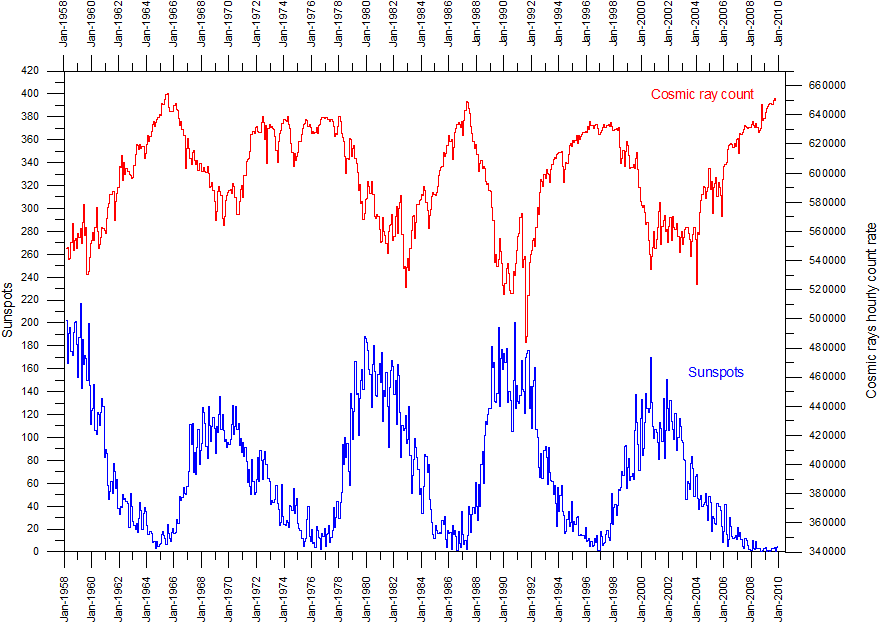
\includegraphics[width=400pt,height=200pt]{img//CosmicRaysAndSunspotsMonthlySince195801.png}
\caption{Inverse relationship with sunspot numbers}
\end{figure}

Signal processing can simplify this problem, traditional signal processing methods can be devided into time-domain methods and frequency-domain methods. Time-domain methods measure max, min, mean values of a signal along time which is easy to understand, but cannot reveal essence of the signal. Frequency-domain decomposes a siganl into a sum of functions according to basis function. Fast Fourier Tansform(FFT) Perhaps the most popular tool for signal processing whose basis function is sinusoidal function. But FFT can not obtain the signal variation of time. As a improvement of FFT, Short Time Fourier Transform(STFT) cotains time information, however, the width of the moving window adopted for the analysis has to be fixed as a function of the minimum frequency of interest, using the best compromise between resolution in both the time and frequency domains\cite{Ditommaso2012}. 

As a time-frequency technique, Empirical Mode Decompisition(EMD) is self-adaptive to dealing with non-stationary and non-linear signals, but it still has "mode mixing" problem. To overcome this problem, we adopt Complete Ensemble Empirical Mode Decomposition with Adaptive Noise (CEEMDAN) in our analysis, CEEMDAN shows good stability in our work. At last, we use the Hilbert transform on the result of CEEMDAN to monitoring intensity change of signal.

\subsection{Empirical Mode Decompisition}
The EMD method is a nonlinear signal transformation procedure introduced by Huang\cite{Huang1998}, this method decomposes a signal into some intrinsic mode function(IMF) through the sfiting process, figure \ref{fig:2} shows the detailed process of sifting process. Each IMF can be obtained from an iterative process of finding the upper and lower envelopes. Cubic-spline is the most popular interpolation method. 

Each IMF satisfies the following two conditions: 
\begin{enumerate}
\item in the whole data set, the number of extrema and the number of zero-crossings must either equal or differ at most by one, and
\item at any point, the mean value of the envelope defined by the local maxima and the envelope defined by the local minima is zero.
\end{enumerate}

For a given signal \(x(t)\), EMD ends up with a representation of the form:
\[ x(t) = r(t) + \sum_{n=1}^N imf_n(t)\]

\(imf_n\)is \(N_{th}\) intrinsic mode function, and \(r(t)\) represents residue corresponding to N intrinsic modes. But EMD has drawback : frequency mixing and un robust, is two figure under same method  

\begin{figure}[h]
      \centering
      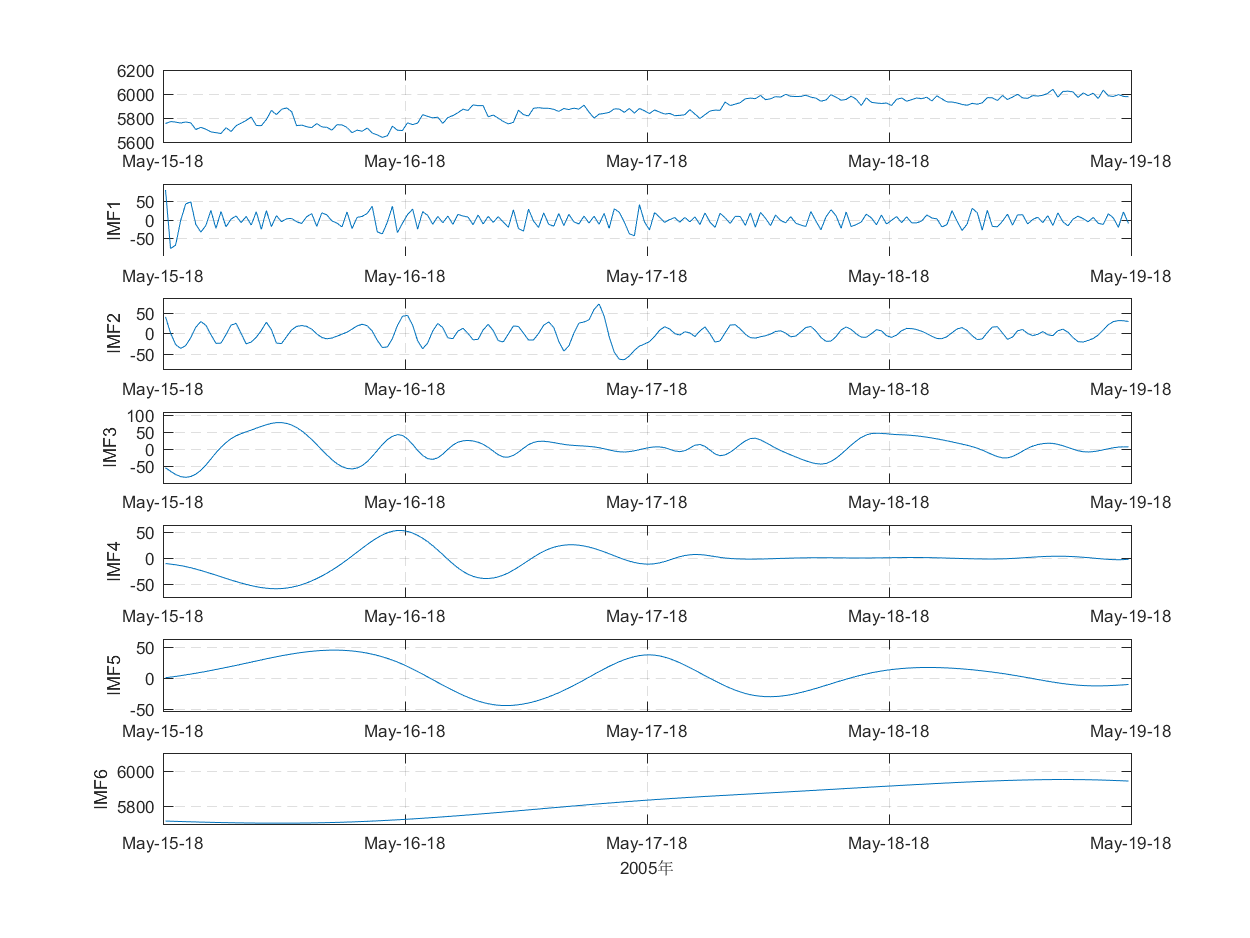
\includegraphics[width=350pt]{img//emd1.png}
      \caption{2005-05-15-18 UTC}\label{fig:3}
      \end{figure}

\begin{figure}[h]
      \centering
      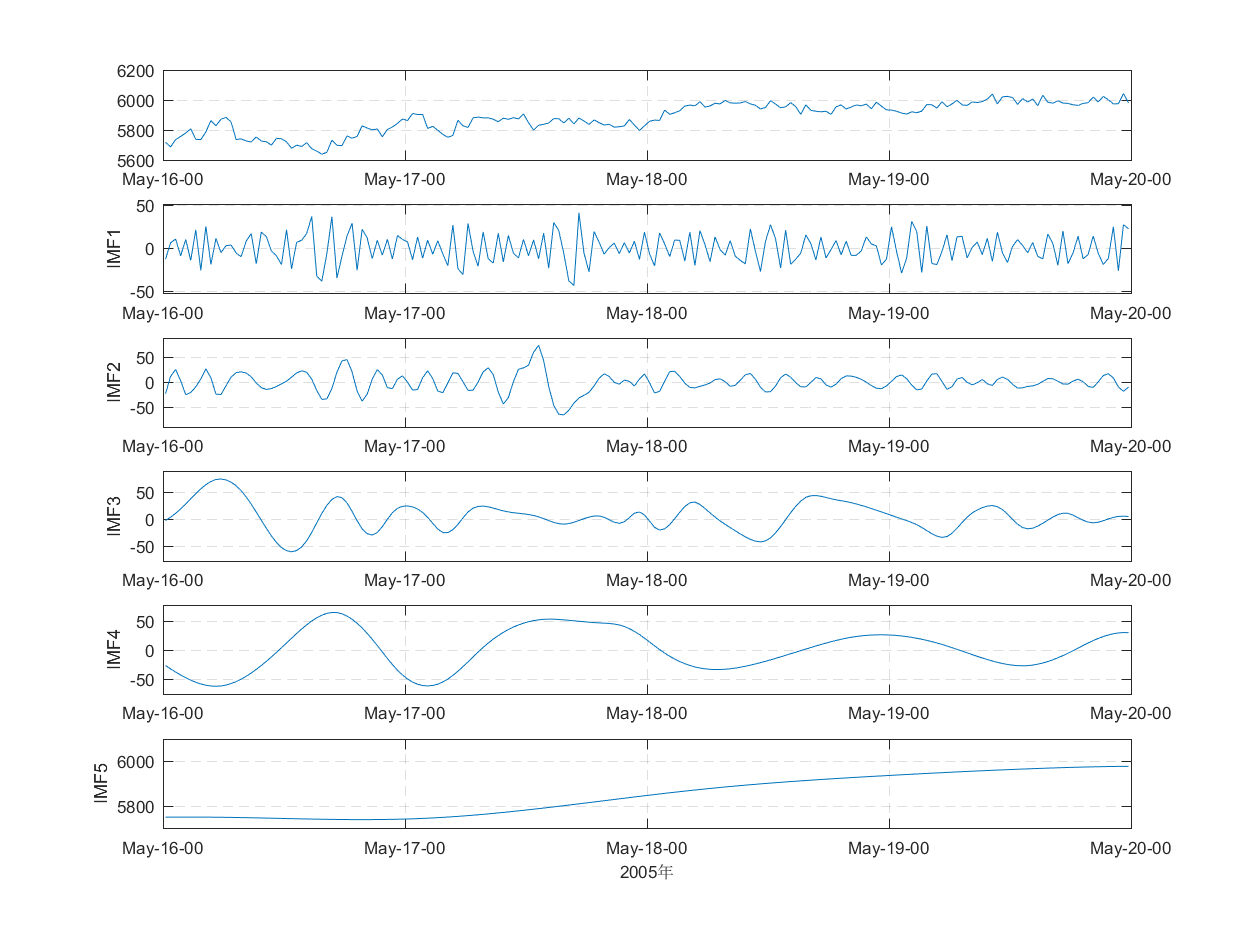
\includegraphics[width=350pt]{img//emd2.png}
      \caption{Process of EMD}\label{fig:4}
      \end{figure}
      
\begin{figure}[h]
      \centering
      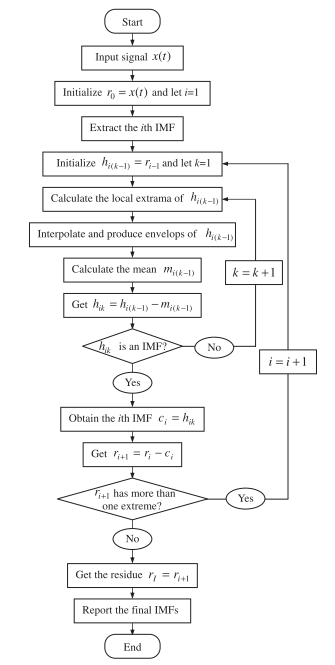
\includegraphics[width=250pt,height=500pt]{img//emd_flowchart.png}
      \caption{Process of EMD}\label{fig:2}
      \end{figure}



\subsection{Complete Ensemble Empirical Mode Decomposition with Adaptive Noise}
A recently demonstrated improved variant of the EMD method is Ensemble EMD (EEMD), inwhichEMD is performed on an ensemble of initial signals, each perturbed by low-amplitude white noise (Wu and Huang 2009). The noise helps the sifting process to avoid mode mixing and to provide more robust and physically meaningful IMFs. In the end the average of the results is designated as the true final result, and thus the direct effect of the noise is canceled out. Computing the EMD of a large ensemble of signals is computationally more intensive, but this difference in computation time can be reduced significantly since the separate ensemble members can be computed in parallel.

Because the added noise does not completely cancel out in the averaging process
for any finite ensemble size, EEMD is no longer a strictly complete decomposition. This issue has been fixed in a EEMD variant called CEEMDAN (Torres et al. 2011). In CEEMDAN, the averaging over all ensemble members is carried separately for each IMF component. By changing the order of averaging over the ensemble and extracting the next IMF, at each point ofthe decomposition procedure the current residual together with the already extracted IMFs sums exactly (or up to numerical precision) to the original signal. This small change also seems to improve the algorithm’s efficiency in recovering an underlying tone from an already noisy input signal (Colominas et al. 2012).

The EMD has great advantages in dealing with non-stationary and non-linear signals, but it still
has “mode mixing” problem. Mode mixing refers to the presence of very similar oscillations in different modes or very disparate amplitude in a mode. By adding Gaussian white noise to the signal, the ensemble empirical mode decomposition (EEMD) algorithm largely eliminates the mode mixing in EMD algorithm[24]. However, the EEMD algorithm cannot completely eliminate Gaussian white noise after signal reconstruction, it cause reconstruction errors. To solve these problems, the complete ensemble empirical mode decomposition with adaptive noise (CEEMDAN) was proposed as an improved version of EEMD[25]. It eliminate mode mixing more effectively, the reconstruction error is almost zero, and the cost of calculation is greatly reduced.

\begin{figure}[h]
      \centering
      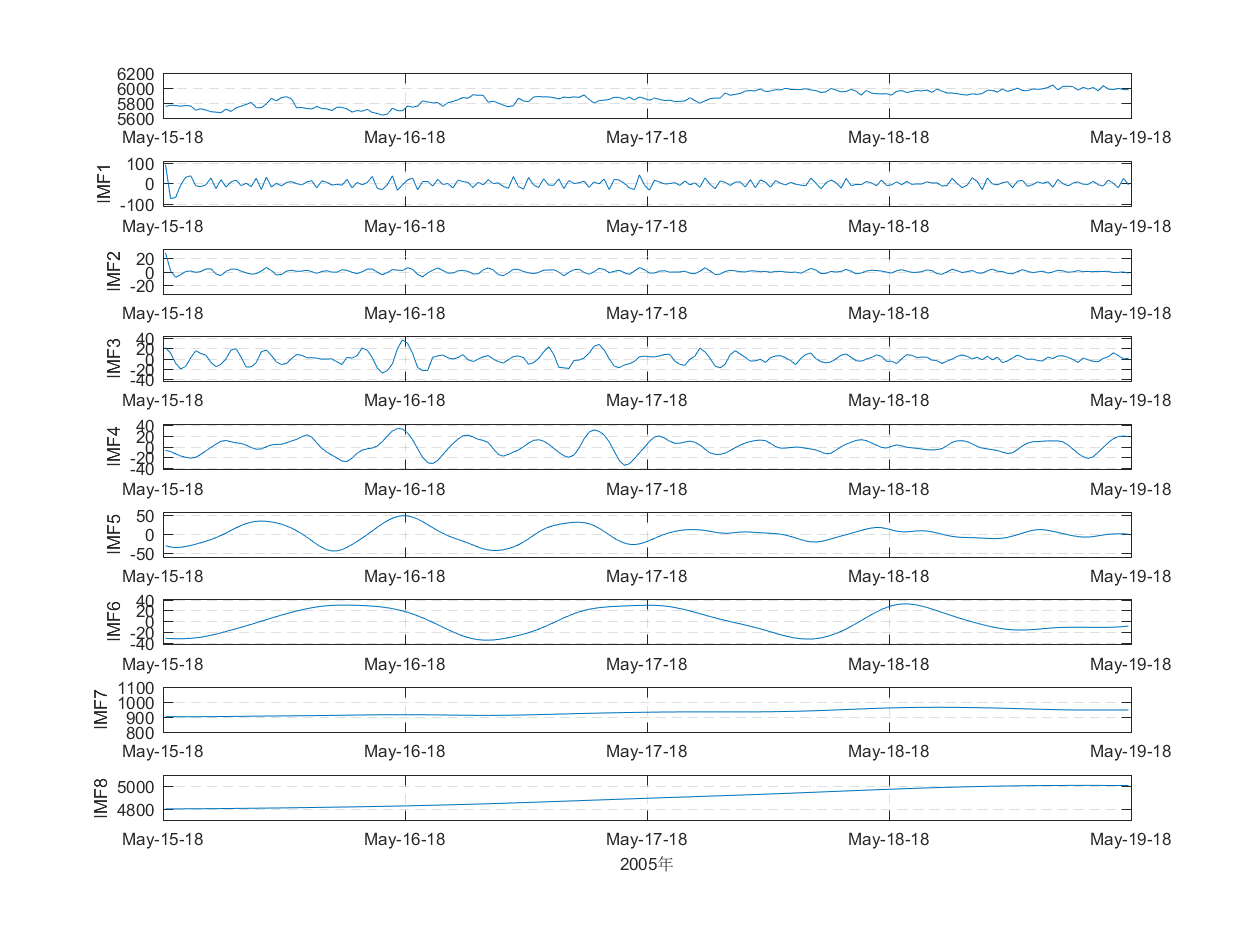
\includegraphics[width=350pt]{img//ceemdan1.png}
      \caption{2005-05-15-18 UTC}\label{fig:5}
      \end{figure}

\begin{figure}[h]
      \centering
      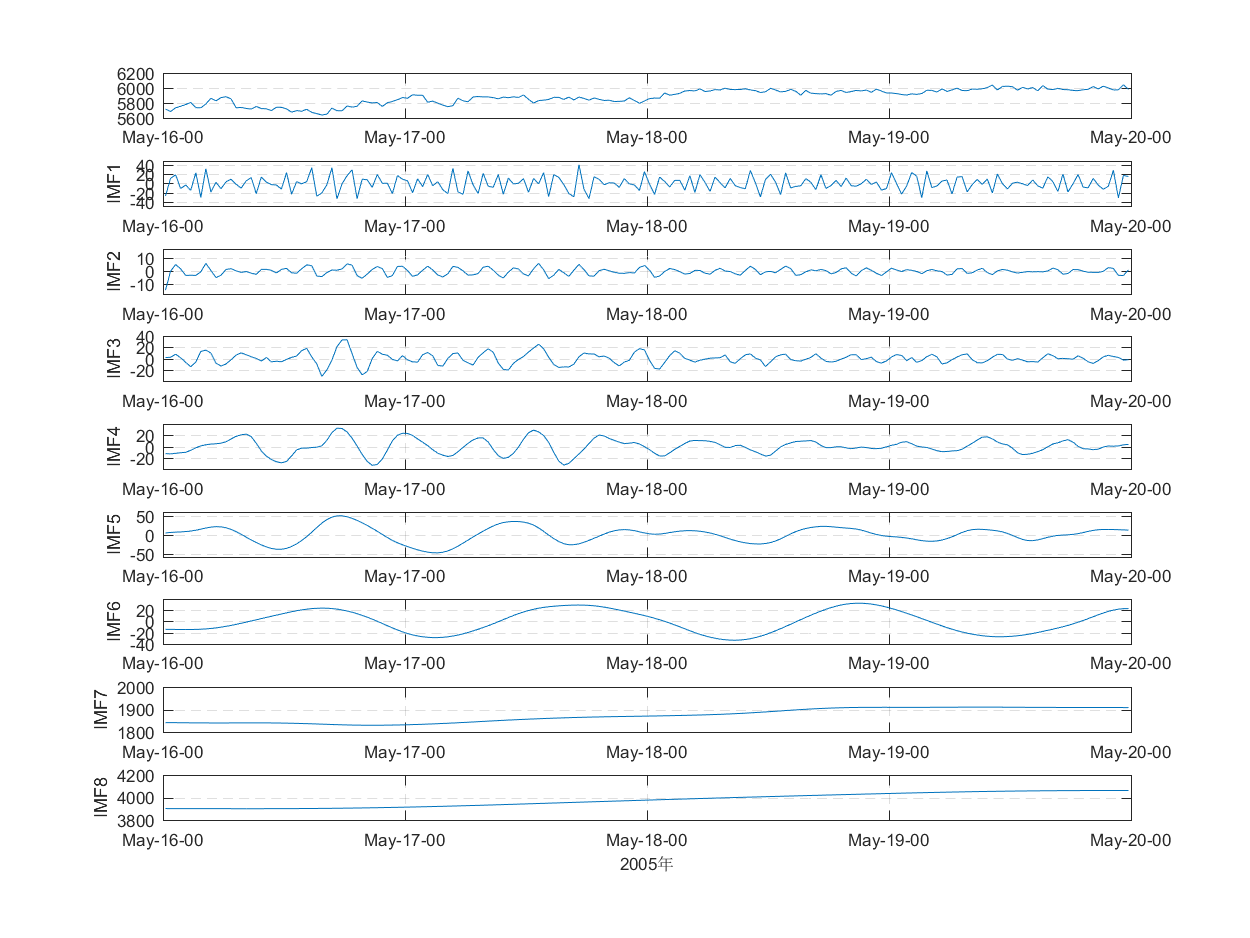
\includegraphics[width=350pt]{img//ceemdan2.png}
      \caption{Process of EMD}\label{fig:6}
      \end{figure}

\subsection{Hilbert Transform}

\subsection{Our Method}
We
\section{Result? Case Study}

\section{Discussion}


%  Numbered lines in equations:
%  To add line numbers to lines in equations,
%  \begin{linenomath*}
%  \begin{equation}
%  \end{equation}
%  \end{linenomath*}



%% Enter Figures and Tables near as possible to where they are first mentioned:
%
% DO NOT USE \psfrag or \subfigure commands.
%
% Figure captions go below the figure.
% Table titles go above tables;  other caption information
%  should be placed in last line of the table, using
% \multicolumn2l{$^a$ This is a table note.}
%
%----------------
% EXAMPLE FIGURES
%
% \begin{figure}
% \includegraphics{example.png}
% \caption{caption}
% \end{figure}
%
% Giving latex a width will help it to scale the figure properly. A simple trick is to use \textwidth. Try this if large figures run off the side of the page.
% \begin{figure}
% \noindent\includegraphics[width=\textwidth]{anothersample.png}
%\caption{caption}
%\label{pngfiguresample}
%\end{figure}
%
%
% If you get an error about an unknown bounding box, try specifying the width and height of the figure with the natwidth and natheight options. This is common when trying to add a PDF figure without pdflatex.
% \begin{figure}
% \noindent\includegraphics[natwidth=800px,natheight=600px]{samplefigure.pdf}
%\caption{caption}
%\label{pdffiguresample}
%\end{figure}
%
%
% PDFLatex does not seem to be able to process EPS figures. You may want to try the epstopdf package.
%

%
% ---------------
% EXAMPLE TABLE
%
% \begin{table}
% \caption{Time of the Transition Between Phase 1 and Phase 2$^{a}$}
% \centering
% \begin{tabular}{l c}
% \hline
%  Run  & Time (min)  \\
% \hline
%   $l1$  & 260   \\
%   $l2$  & 300   \\
%   $l3$  & 340   \\
%   $h1$  & 270   \\
%   $h2$  & 250   \\
%   $h3$  & 380   \\
%   $r1$  & 370   \\
%   $r2$  & 390   \\
% \hline
% \multicolumn{2}{l}{$^{a}$Footnote text here.}
% \end{tabular}
% \end{table}

%% SIDEWAYS FIGURE and TABLE
% AGU prefers the use of {sidewaystable} over {landscapetable} as it causes fewer problems.
%
% \begin{sidewaysfigure}
% \includegraphics[width=20pc]{figsamp}
% \caption{caption here}
% \label{newfig}
% \end{sidewaysfigure}
%
%  \begin{sidewaystable}
%  \caption{Caption here}
% \label{tab:signif_gap_clos}
%  \begin{tabular}{ccc}
% one&two&three\\
% four&five&six
%  \end{tabular}
%  \end{sidewaystable}

%% If using numbered lines, please surround equations with \begin{linenomath*}...\end{linenomath*}
%\begin{linenomath*}
%\begin{equation}
%y|{f} \sim g(m, \sigma),
%\end{equation}
%\end{linenomath*}

%%% End of body of article

%%%%%%%%%%%%%%%%%%%%%%%%%%%%%%%%
%% Optional Appendix goes here
%
% The \appendix command resets counters and redefines section heads
%
% After typing \appendix
%
%\section{Here Is Appendix Title}
% will show
% A: Here Is Appendix Title
%
%\appendix
%\section{Here is a sample appendix}

%%%%%%%%%%%%%%%%%%%%%%%%%%%%%%%%%%%%%%%%%%%%%%%%%%%%%%%%%%%%%%%%
%
% Optional Glossary, Notation or Acronym section goes here:
%
%%%%%%%%%%%%%%
% Glossary is only allowed in Reviews of Geophysics
%  \begin{glossary}
%  \term{Term}
%   Term Definition here
%  \term{Term}
%   Term Definition here
%  \term{Term}
%   Term Definition here
%  \end{glossary}

%
%%%%%%%%%%%%%%
% Acronyms
%   \begin{acronyms}
%   \acro{Acronym}
%   Definition here
%   \acro{EMOS}
%   Ensemble model output statistics
%   \acro{ECMWF}
%   Centre for Medium-Range Weather Forecasts
%   \end{acronyms}

%
%%%%%%%%%%%%%%
% Notation
%   \begin{notation}
%   \notation{$a+b$} Notation Definition here
%   \notation{$e=mc^2$}
%   Equation in German-born physicist Albert Einstein's theory of special
%  relativity that showed that the increased relativistic mass ($m$) of a
%  body comes from the energy of motion of the body—that is, its kinetic
%  energy ($E$)—divided by the speed of light squared ($c^2$).
%   \end{notation}




%%%%%%%%%%%%%%%%%%%%%%%%%%%%%%%%%%%%%%%%%%%%%%%%%%%%%%%%%%%%%%%%
%
%  ACKNOWLEDGMENTS
%
% The acknowledgments must list:
%
% >>>>	A statement that indicates to the reader where the data
% 	supporting the conclusions can be obtained (for example, in the
% 	references, tables, supporting information, and other databases).
%
% 	All funding sources related to this work from all authors
%
% 	Any real or perceived financial conflicts of interests for any
%	author
%
% 	Other affiliations for any author that may be perceived as
% 	having a conflict of interest with respect to the results of this
% 	paper.
%
%
% It is also the appropriate place to thank colleagues and other contributors.
% AGU does not normally allow dedications.


\acknowledgments
Enter acknowledgments, including your data availability statement, here.


%% ------------------------------------------------------------------------ %%
%% References and Citations

%%%%%%%%%%%%%%%%%%%%%%%%%%%%%%%%%%%%%%%%%%%%%%%
%
% \bibliography{<name of your .bib file>} don't specify the file extension
%
% don't specify bibliographystyle
%%%%%%%%%%%%%%%%%%%%%%%%%%%%%%%%%%%%%%%%%%%%%%%

\bibliography{biblio-u1}



%Reference citation instructions and examples:
%
% Please use ONLY \cite and \citeA for reference citations.
% \cite for parenthetical references
% ...as shown in recent studies (Simpson et al., 2019)
% \citeA for in-text citations
% ...Simpson et al. (2019) have shown...
%
%
%...as shown by \citeA{jskilby}.
%...as shown by \citeA{lewin76}, \citeA{carson86}, \citeA{bartoldy02}, and \citeA{rinaldi03}.
%...has been shown \cite{jskilbye}.
%...has been shown \cite{lewin76,carson86,bartoldy02,rinaldi03}.
%... \cite <i.e.>[]{lewin76,carson86,bartoldy02,rinaldi03}.
%...has been shown by \cite <e.g.,>[and others]{lewin76}.
%
% apacite uses < > for prenotes and [ ] for postnotes
% DO NOT use other cite commands (e.g., \citet, \citep, \citeyear, \nocite, \citealp, etc.).
%



\end{document}



More Information and Advice:

%% ------------------------------------------------------------------------ %%
%
%  SECTION HEADS
%
%% ------------------------------------------------------------------------ %%

% Capitalize the first letter of each word (except for
% prepositions, conjunctions, and articles that are
% three or fewer letters).

% AGU follows standard outline style; therefore, there cannot be a section 1 without
% a section 2, or a section 2.3.1 without a section 2.3.2.
% Please make sure your section numbers are balanced.
% ---------------
% Level 1 head
%
% Use the \section{} command to identify level 1 heads;
% type the appropriate head wording between the curly
% brackets, as shown below.
%
%An example:
%\section{Level 1 Head: Introduction}
%
% ---------------
% Level 2 head
%
% Use the \subsection{} command to identify level 2 heads.
%An example:
%\subsection{Level 2 Head}
%
% ---------------
% Level 3 head
%
% Use the \subsubsection{} command to identify level 3 heads
%An example:
%\subsubsection{Level 3 Head}
%
%---------------
% Level 4 head
%
% Use the \subsubsubsection{} command to identify level 3 heads
% An example:
%\subsubsubsection{Level 4 Head} An example.
%
%% ------------------------------------------------------------------------ %%
%
%  IN-TEXT LISTS
%
%% ------------------------------------------------------------------------ %%
%
% Do not use bulleted lists; enumerated lists are okay.
% \begin{enumerate}
% \item
% \item
% \item
% \end{enumerate}
%
%% ------------------------------------------------------------------------ %%
%
%  EQUATIONS
%
%% ------------------------------------------------------------------------ %%

% Single-line equations are centered.
% Equation arrays will appear left-aligned.

Math coded inside display math mode \[ ...\]
 will not be numbered, e.g.,:
 \[ x^2=y^2 + z^2\]

 Math coded inside \begin{equation} and \end{equation} will
 be automatically numbered, e.g.,:
 \begin{equation}
 x^2=y^2 + z^2
 \end{equation}


% To create multiline equations, use the
% \begin{eqnarray} and \end{eqnarray} environment
% as demonstrated below.
\begin{eqnarray}
  x_{1} & = & (x - x_{0}) \cos \Theta \nonumber \\
        && + (y - y_{0}) \sin \Theta  \nonumber \\
  y_{1} & = & -(x - x_{0}) \sin \Theta \nonumber \\
        && + (y - y_{0}) \cos \Theta.
\end{eqnarray}

%If you don't want an equation number, use the star form:
%\begin{eqnarray*}...\end{eqnarray*}

% Break each line at a sign of operation
% (+, -, etc.) if possible, with the sign of operation
% on the new line.

% Indent second and subsequent lines to align with
% the first character following the equal sign on the
% first line.

% Use an \hspace{} command to insert horizontal space
% into your equation if necessary. Place an appropriate
% unit of measure between the curly braces, e.g.
% \hspace{1in}; you may have to experiment to achieve
% the correct amount of space.


%% ------------------------------------------------------------------------ %%
%
%  EQUATION NUMBERING: COUNTER
%
%% ------------------------------------------------------------------------ %%

% You may change equation numbering by resetting
% the equation counter or by explicitly numbering
% an equation.

% To explicitly number an equation, type \eqnum{}
% (with the desired number between the brackets)
% after the \begin{equation} or \begin{eqnarray}
% command.  The \eqnum{} command will affect only
% the equation it appears with; LaTeX will number
% any equations appearing later in the manuscript
% according to the equation counter.
%

% If you have a multiline equation that needs only
% one equation number, use a \nonumber command in
% front of the double backslashes (\\) as shown in
% the multiline equation above.

% If you are using line numbers, remember to surround
% equations with \begin{linenomath*}...\end{linenomath*}

%  To add line numbers to lines in equations:
%  \begin{linenomath*}
%  \begin{equation}
%  \end{equation}
%  \end{linenomath*}



